\section[Normalisation]{Normalisation}

%\subsection{Règles de normalisations}

\begin{frame}
  \frametitle{Bonnes pratiques}
  \begin{itemize}
    \item Un bon schéma entités-associations doit répondre à 9 règles de normalisation:
      \begin{enumerate}
        \item Normalisation des entités
        \item Normalisation des noms
        \item Normalisation des identifiants
        \item Normalisation des attributs
        \item Normalisation des associations
        \item Normalisation des cardinalités
        \item Première forme normale
        \item Deuxième forme normale
        \item Troisième forme normale
      \end{enumerate}
  \end{itemize}
\end{frame}

\begin{frame}
  \frametitle{Normalisation des entités}
  \begin{itemize}
    \item Toutes les entités qui sont remplaçables par une association doivent être remplacées
  \end{itemize}
\end{frame}


\begin{frame}
  \frametitle{Normalisation des noms (1)}
  \begin{itemize}
    \item Le nom d'une entité, d'une association ou d'un attribut doit être unique
    \item Conseils :
      \begin{itemize}
        \item Pour les entités, utiliser un nom commun au pluriel (ex : clients)
        \item Pour les associations, utiliser un verbe à l'infinitif (ex : effectuer, concerner)
          éventuellement à la forme passive (être commandé) et accompagné d'un adverbe (avoir lieu dans,
          pendant, à)
        \item Pour les attributs, utiliser un nom commun singulier (ex : nom, numéro, libellé,
          description), éventuellement accompagné du nom de l'entité ou de l'association dans laquelle il se
          trouve (ex : nom de client, numéro d'article)
      \end{itemize}
    \item Remarque : lorsqu'il reste plusieurs fois le même nom, c'est parfois symptomatique d'une modélisation qui
      n'est pas terminée
  \end{itemize}
\end{frame}

\begin{frame}
  \frametitle{Normalisation des noms (2)}
  \begin{itemize}
    \item Deux entités homogènes peuvent être fusionnées
  \end{itemize}
  \begin{center}
    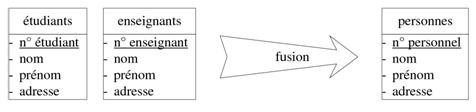
\includegraphics[width=0.8\linewidth]{fusion_entites.jpg}
  \end{center}
\end{frame}

\begin{frame}
  \frametitle{Normalisation des noms (3)}
  \begin{itemize}
    \item Éviter les redondances : gaspillage d'espace et risque incohérence
  \end{itemize}
  \begin{center}
    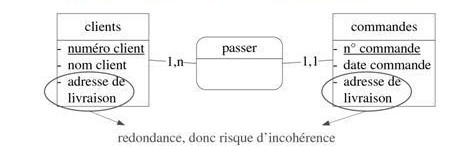
\includegraphics[width=0.8\linewidth]{redondance_attributs.jpg}
  \end{center}
  \begin{itemize}
    \item Si les adresses ne sont pas les mêmes, où faut-il livrer ?
  \end{itemize}
\end{frame}

\begin{frame}
  \frametitle{Normalisation des identifiants}
  \begin{itemize}
    \item Chaque entité doit posséder un identifiant
    \item Conseils :
      \begin{itemize}
        \item Éviter les identifiants composés de plusieurs attributs (ex : nom et prénom) : mauvaises
          performances et problème d'unicité possible
        \item Préférer un identifiant court pour une recherche plus rapide (éviter notamment les chaînes de
          caractères complexes)
        \item Éviter les identifiants susceptibles de changer au cours du temps (ex : les plaques d'immatriculation)
      \end{itemize}
    \item Conclusion : en général, l'identifiant est un entier, souvent incrémenté automatiquement
  \end{itemize}
\end{frame}

\begin{frame}
  \frametitle{Normalisation des attributs (1)}
  \begin{itemize}
    \item Remplacer les attributs en plusieurs exemplaires en une association supplémentaire de cardinalités
      maximales $n$
  \end{itemize}
  \begin{center}
    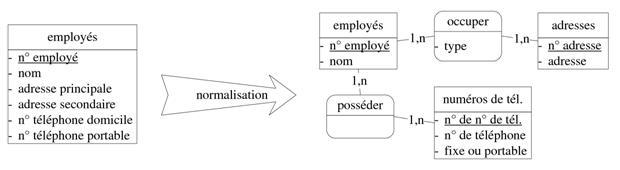
\includegraphics[width=0.9\linewidth]{normalisation_attributs.jpg}
  \end{center}
  \begin{itemize}
    \item Problème d'évolutivité des attributs en plusieurs exemplaires : comment faire si un employé a deux
      adresses secondaires ?
  \end{itemize}
\end{frame}

\begin{frame}
  \frametitle{Normalisation des attributs (2)}
  \begin{itemize}
    \item Ne pas avoir d'attribut calculable à partir d'autres attributs
  \end{itemize}
  \begin{center}
    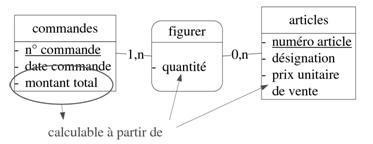
\includegraphics[width=0.6\linewidth]{attribut_calculable.jpg}
  \end{center}
  \begin{itemize}
    \item Risque d'incohérence entre les valeurs des attributs de base et celles des attributs calculés
    \item Attributs calculables classiques à éviter:
      \begin{itemize}
        \item l'âge : calculable à partir de la date de naissance
        \item le département : calculable à partir du code postal
      \end{itemize}
  \end{itemize}
\end{frame}

\begin{frame}
  \frametitle{Normalisation des attributs des associations (1)}
  \begin{itemize}
    \item Les attributs d'une association doivent dépendre directement des identifiants de toutes les entités
      en association
  \end{itemize}
  \begin{center}
    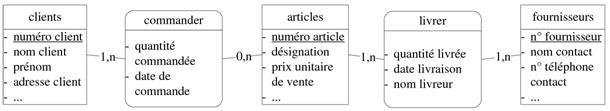
\includegraphics[width=0.9\linewidth]{cardinalites.jpg}
  \end{center}
  \begin{itemize}
    \item La quantité commandée dépend de numéro de client et du numéro d'article, la date de commande non
    \item[$\ra$] Création d'une entité commandes (idem pour les livraisons)
  \end{itemize}
\end{frame}

\begin{frame}
  \frametitle{Normalisation des attributs des associations (2)}
  \begin{itemize}
    \item Les attributs d'une association doivent dépendre directement des identifiants de toutes les entités
      en association
  \end{itemize}
  \begin{center}
    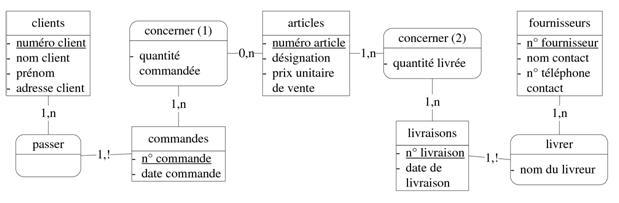
\includegraphics[width=0.9\linewidth]{normalisation_attributs_associations.jpg}
  \end{center}
  \begin{itemize}
    \item La quantité commandée dépend de numéro de client et du numéro d'article, la date de commande non
    \item[$\ra$] Création d'une entité commandes (idem pour les livraisons)
  \end{itemize}
\end{frame}

\begin{frame}
  \frametitle{Normalisation des attributs des associations (3)}
  \begin{itemize}
    \item Une entité avec une cardinalité de 1,1 ou 0,1 aspire les attributs de l'association
  \end{itemize}
  \begin{center}
    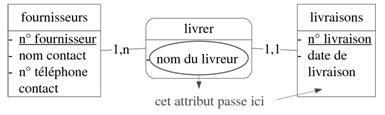
\includegraphics[width=0.6\linewidth]{normalisation_attribut_association.jpg}
  \end{center}
\end{frame}

\begin{frame}
  \frametitle{Normalisation des associations (1)}
  \begin{itemize}
    \item On élimine les associations fantômes, redondantes ou en plusieurs exemplaires
  \end{itemize}
  \begin{center}
    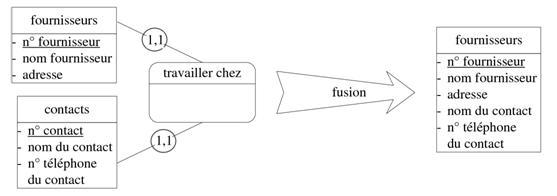
\includegraphics[width=0.9\linewidth]{association_fantome.jpg}
  \end{center}
  \begin{itemize}
    \item Les cardinalités sont toutes 1,1 donc c'est une association fantôme
  \end{itemize}
\end{frame}

\begin{frame}
  \frametitle{Normalisation des associations (2)}
  \begin{itemize}
    \item Les associations redondantes signifient qu'il existe deux chemins pour aller d'une entité à une autre :
      \begin{itemize}
        \item Ils doivent avoir deux significations ou deux durées de vie différentes
        \item Ou le chemin le plus court doit être supprimé
      \end{itemize}
  \end{itemize}
  \begin{center}
    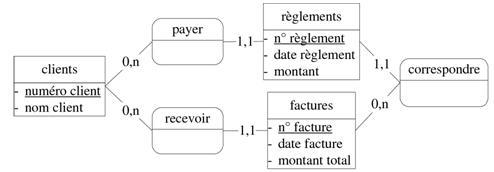
\includegraphics[width=0.9\linewidth]{association_redondante.jpg}
  \end{center}
  \begin{itemize}
    \item Si un client ne peut pas régler la facture d'un autre client, alors l'association payer est inutile
    \item[$\ra$] Elle doit être supprimée
  \end{itemize}
\end{frame}

\begin{frame}
  \frametitle{Normalisation des associations (3)}
  \begin{itemize}
    \item Les associations en plusieurs exemplaires doivent, si elle le peuvent, être regroupée
      \begin{itemize}
        \item Évolutivité : on privilégie les cardinalités maximales $n$
        \item Une cadinalité minimale de plus de $1$ est inutile si la cardinalité maximale est $n$
      \end{itemize}
  \end{itemize}
  \begin{center}
    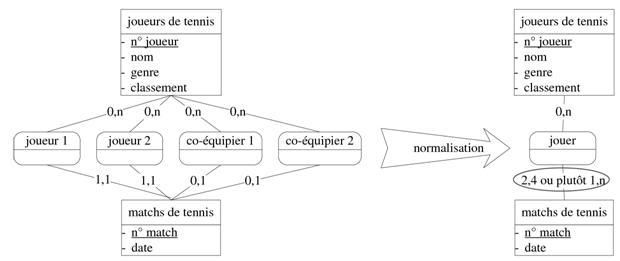
\includegraphics[width=0.9\linewidth]{association_plusieurs_exemplaires.jpg}
  \end{center}
  \begin{itemize}
    \item Une association suffit pour remplacer les 4 associations
  \end{itemize}
\end{frame}

%\subsection{Les formes normales}

\begin{frame}
  \frametitle{Première forme normale}
  \begin{itemize}
    \item «~Tous les attributs doivent posséder une valeur sémantiquement
        atomique.~»
    \item Conséquence : à un instant donné un attribut ne peut prendre qu'une
        valeur et non pas, un ensemble ou une liste de valeurs
  \end{itemize}
  \begin{center}
    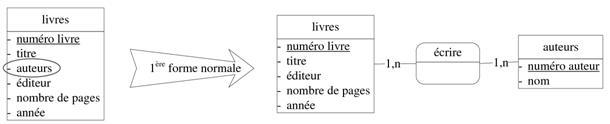
\includegraphics[width=0.9\linewidth]{premiere_forme_normale.jpg}
  \end{center}
  \begin{itemize}
    \item Si un attribut prend plusieurs valeurs, alors ces valeurs doivent faire l'objet d'une entité
      supplémentaire, en association avec la première
  \end{itemize}
\end{frame}

\begin{frame}
  \frametitle{Deuxième forme normale}
  \begin{itemize}
    \item «~En première forme normale et :\\
        Un attribut non identifiant ne dépend pas d’une partie de l'identifiant
        mais de tout l'identifiant~»
    \item Cela peut arriver si l'identifiant est composé de plusieurs attributs
    \item[$\ra$] Peut être oubliée si l'on utilise des identifiants non composés et de type entier
  \end{itemize}
\end{frame}

\begin{frame}
  \frametitle{Troisième forme normale}
  \begin{itemize}
    \item «~En deuxième forme normale et :\\
        Tous les attributs non identifiants doivent dépendre directement de
        l'identifiant~»
    \item En pratique on utilise la troisième forme normale de Boyce-Codd, plus complète
  \end{itemize}
\end{frame}

\begin{frame}
  \frametitle{Troisième forme normale de Boyce-Codd (1)}
  \begin{itemize}
    \item «~En deuxième forme normale et :
        \begin{itemize}
            \item Tous les attributs non identifiants doivent dépendre directement de l'identifiant
            \item Aucune partie de l'identifiant dépend d'un attribut
                non-identifiant~»
        \end{itemize}
  \end{itemize}
\end{frame}

\begin{frame}
  \frametitle{Troisième forme normale de Boyce-Codd (2)}
  \begin{itemize}
    \item Version simplifié : tous les attributs d'une entité doivent dépendre directement de son identifiant
      et d'aucun autre attribut
    \item Si ce n'est pas le cas, il faut placer l'attribut pathologique dans une entité séparée en
      association avec la première
  \end{itemize}
  \begin{tabular}{c | c | c | c | c }
    numéro avion & constructeur & modèle & capacité & propriétaire \\
    \hline \hline
    1 & Airbus & 380 & 180 & Air France \\
    2 & Boeing & 747 & 314 & British Airways \\
    3 & Airbus & 380 & 180 & KLM
  \end{tabular}
  \begin{itemize}
    \item Redondance ($\ra$ risque d'incohérence) pour les colonnes constructeur
        et capacité qui dépendent de modèle
  \end{itemize}
\end{frame}

\begin{frame}
  \frametitle{Troisième forme normale de Boyce-Codd (3)}
  \begin{itemize}
    \item Version simplifié : tous les attributs d'une entité doivent dépendre directement de son identifiant et d'aucun autre
      attribut
    \item Si ce n'est pas le cas, il faut placer l'attribut pathologique dans une entité séparée en
      association avec la première
  \end{itemize}
  \begin{center}
    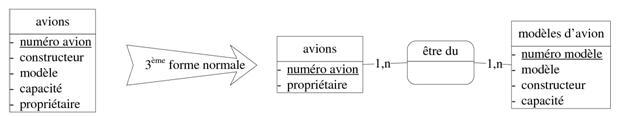
\includegraphics[width=0.9\linewidth]{troisieme_forme_normale.jpg}
  \end{center}
  \begin{itemize}
    \item La colonne constructeur devrait également être dans une entité séparée constructeurs (en association avec modèles d'avion)
  \end{itemize}
\end{frame}

